\chapter{{\color{done}Орографические координаты}}

\begin{warn}
    Не забыть добавить аналоги в сферических координатах!
\end{warn}

\section{{\color{done}Уравнения гидротермодинамики в сигма системе координат}}

В связи с тем, что хотя в $z$-системе граничные условия прозрачны, но область интегрирования становится в условиях рельефа крайне сложной, а $p$-система не вполне естественна для постановки условий на нижней границе, выход из сложившейся ситуации ищут в создании так называемых орографических координат, в которых область приобрела бы простую геометрию, удобную для численного решения уравнений гидротермодинамики, и которая была бы естественной с точки зрения постановки условий на нижней границе.

Применительно к $p$-системе координат, используется так называемая сигма-система координат, в которой вместо давления вводится некоторая безразмерная переменная. Наиболее часто употребляются следующие две формы $\sigma$-координат: 

\begin{equation}
\label{eq:sigma}
    \sigma=\frac{p}{p_s},
\end{equation}
где $p$ -- некоторое текущее давление, $p_s$-давление на поверхности Земли и несколько отличная формулировка $\sigma$-координаты:
\begin{equation}
    \sigma=\frac{p-p_T}{p_s-p_T},
\end{equation}
где $p_s$-давление у поверхности Земли, $p_T$-давление на верхней границе области интегрирования, $p$-текущее давление. Нетрудно заметить, что в последнем, наиболее употребительном варианте записи $\sigma$-координаты, она изменяется в пределах $0\leq\sigma\leq1$. В плоском случае $\sigma$-координаты выглядит так, как показано на рис. $\ref{fig:ch9.1}$.

    % \begin{figure}[h]
    % \centering
    % 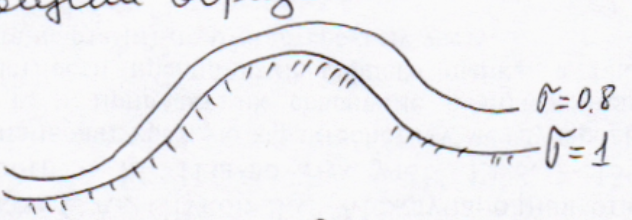
\includegraphics[width=0.9\linewidth]{pics/ch9.1.png}
    % \caption{\label{fig:ch9.1}
    %  $\sigma$-координата
    % }
    % \end{figure}    

    \begin{figure}[h]
        \centering
        % 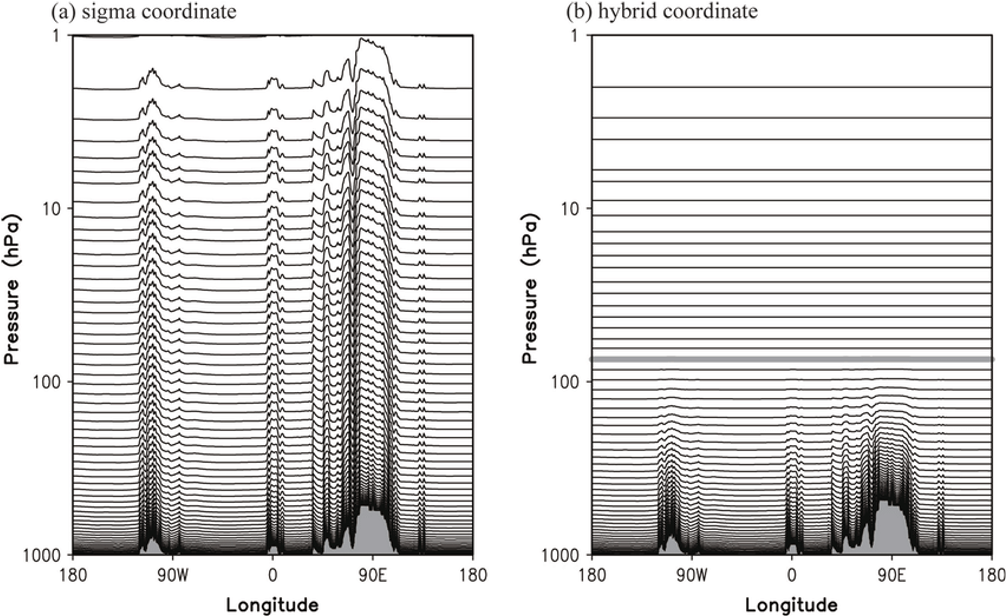
\includegraphics[width=0.9\linewidth]{pics/ch9.3.png}
        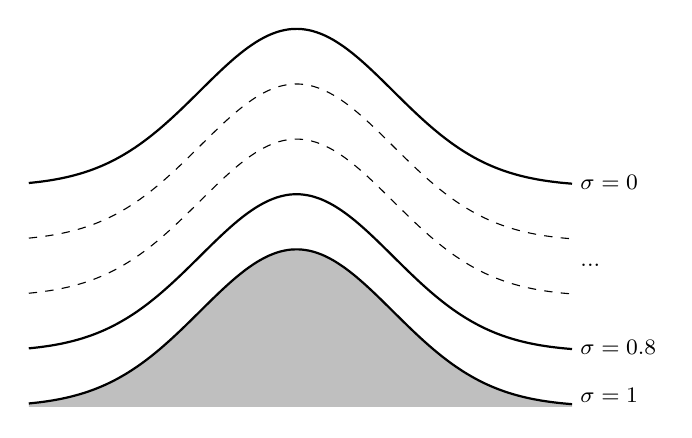
\begin{tikzpicture}[declare function={g(\x)=2*exp(-\x*\x/3);
            xmax=3.5;xmin=-3.4;x0=1.5;ymax=2.75;}]
             % \draw[gray!50] ;
             \footnotesize
             \fill[gray!50] plot[domain=xmin:xmax,samples=15,smooth] (\x,{g(\x)}) -- (xmax,0) -| cycle;  
             % \draw[pattern=grid]   plot[domain=xmin:xmax,samples=51,smooth] (\x,{g(\x)}); 
             \draw[thick]   plot[domain=xmin:xmax,samples=51,smooth] (\x,{g(\x)}); 
             \draw[thick]   plot[domain=xmin:xmax,samples=51,smooth] (\x,{0.7+g(\x)}); 
             \draw[dashed]  plot[domain=xmin:xmax,samples=51,smooth] (\x,{1.4+g(\x)}); 
             \draw[dashed]  plot[domain=xmin:xmax,samples=51,smooth] (\x,{2.1+g(\x)}); 
             \draw[thick]   plot[domain=xmin:xmax,samples=51,smooth] (\x,{2.8+g(\x)}); 
             \draw (xmax,0.15) node[right] {$\sigma=1$} ;
             \draw (xmax,0.75) node[right] {$\sigma=0.8$} ;
             \draw (xmax,1.80) node[right] {...} ;
             \draw (xmax,2.85) node[right] {$\sigma=0$} ;
        \end{tikzpicture}
        \caption{\label{fig:ch9.1} $\sigma$-координата}
    \end{figure}    

То есть $\sigma$-поверхности в трехмерном случае в первом приближении повторяют рельеф (небольшие отклонения вследствие изменчивости поля давления, конечно, имеются).

Аналогичная орографическая координата имеется и для $z$-системы: $\eta=\frac{z-z_s}{z_T-z_s}$, которая также изменяется в пределах $0\leq\eta\leq1$.

Поскольку эта система координат широко используется как при численном прогнозировании погоды, так и в исследовательских задачах, мы остановимся на выводе уравнений в $\sigma$-системе более подробно. Эта система ортогональна, но недостаток ее состоит в том, что искривленные рельефом $\sigma$-поверхности сохраняют это свойство во всей области интегрирования. На уровне $\sigma=1$ перевод переменных из координат $(x,y,p_s)$, в координаты $(x,y,\sigma)$ не представляет проблем: все наземные наблюдения находятся на уровне $\sigma=1$, но в свободной атмосфере все наблюдения на изобарических поверхностях (в $p$-системе), поэтому приходится неизбежно производить переинтерполяцию наблюдений из $p$-координат в $\sigma$-систему. Естественно, что такого рода интерполяции вносят дополнительные ошибки. С тем, чтобы уменьшить такого рода ошибки в последнее время наметился переход к некоторым гибридным системам координат, в которых осуществляется постепенный переход от $\sigma$-поверхностей вблизи Земли к $p$-поверхностям в свободной атмосфере с тем, чтобы уменьшить отмеченные много выше отрицательные эффекты. 

Итак переходим к преобразованию уравнений из $p$-системы в $\sigma$-систему. Далее все координаты, снабженные индексом $p$ будет обозначать их принадлежность к $p$-системе, а индекс $\sigma$ -- к сигма системе. Для простоты вывод будет производиться для варианта $\sigma=\frac{p}{p_s}$.  Для другого варианта промежуточные выкладки будут опущены. Будем считать, что помимо $\sigma=\frac{p}{p_s}$ координатам этой системы являются: 
\begin{equation}
    x_{\sigma}=x_p=x; \:\:y_{\sigma}=y_p=y; \:\:t_{\sigma}=t_p=t
\end{equation}
Для перехода от $p$-системы к $\sigma$-системе нам нужно будет выполнить дифференцирование сложной функции нескольких переменных. Вспомним правило дифференцирования сложной функции $u=f(x,y,...,t)$, где $x=\varphi(\xi)$, $y=\psi(\xi)$, ..., $t=\chi(\xi)$.
\begin{equation}
\label{eq:pdsf}
    \pd{u}{\xi}=\pd{u}{x}\pd{x}{\xi}+\pd{u}{y}\pd{y}{\xi}+\cdots+\pd{u}{t}\pd{t}{\xi}
\end{equation}
Так как для нас исходными буду служить операторы и переменные в $p$-системе и наша задача состоит в получении этих операторов в поле новых переменных, то роль переменной $\xi$ мы отведем координатам в $p$-системе, а роль переменных $x$, $y$, ..., $t$ -- координатам в $\sigma$-системе, то есть для наших конкретных переменных в $\sigma$-системе координат будем иметь
\begin{equation*}
    u=f(x_{\sigma},y_{\sigma},\sigma,t_{\sigma}).
\end{equation*}
Если для простоты рассмотрим случай идеальной жидкости (не будем учитывать вязкие члены), то нашими стандартными операторами будут $\pd{}{x_p}$, $\pd{}{y_p}$, $\pd{}{p}$ и $\pd{}{t_p}$. Начнем с использования (\ref{eq:pdsf}) искать соответствие этим операторам в $\sigma$-системе. Начнем с оператора $\pd{}{x_p}$.

\begin{warn}
    Привести в порядок текст ниже. Тут то в общем виде написано, то для $u$. 
\end{warn}

Будем иметь
\begin{equation*}
    \pd{u}{x_p}=
     \pd{u}{x_{\sigma}} \cancelto{1}{ \pd{x_{\sigma}}{x_p} }+
    \pd{u}{y_{\sigma}}\cancelto{0}{\pd{y_{\sigma}}{x_p}}+
    \pd{u}{\sigma}\pd{\sigma}{x_p}+
    \pd{u}{t_{\sigma}}\cancelto{0}{\pd{t_{\sigma}}{x_p}}.
\end{equation*}
Часть из полученных слагаемых равно нулю, т.к. в них выходят множители, не зависящие от координаты $x_p$. Учитывая дополнительно, что по условию $x_{\sigma}=x_p$, получим
\begin{multline*}
    \pd{u}{x_p}=\pd{u}{x_{\sigma}}+
        \pd{u}{\sigma}\pd{}{x_p} \left[ \frac{p}{p_s} \right] = 
        \pd{u}{x_{\sigma}}+
        \pd{u}{\sigma} \left[ \frac{ \cancelto{0}{\pd{p}{x_p}}p_s - p\pd{p_s}{x_p} } { {p_s}^2 } \right] = \\
        = \pd{u}{x_{\sigma}} + 
        \pd{u}{\sigma} \left[ -\frac{p}{{p_s}^2} \pd{p_s}{x_p} \right] = 
        \pd{u}{x_{\sigma}} - \frac{\sigma}{p_s}\pd{p_s}{x_p}\pd{u}{\sigma},
\end{multline*}
откуда
\begin{equation}
    \label{eq:sigma2px}
    \pd{}{x_p}=\pd{}{x_{\sigma}}-\frac{\sigma}{p_s}\pd{p_s}{x_p}\pd{}{\sigma}.
\end{equation}
Аналогичным образом получим 
\begin{equation}
    \label{eq:sigma2py}
    \pd{}{y_p}=\pd{}{y_{\sigma}}-\frac{\sigma}{p_s}\pd{p_s}{y_p}\pd{}{\sigma},
\end{equation}
\begin{equation}
    \label{eq:sigma2pp}
    \pd{}{p}= \frac{1}{p_s}\pd{}{\sigma}.
\end{equation}
Так как от $t$ зависит только $\sigma$ и $t_p$, то для производной по времени будем иметь
\begin{equation*}
    \pd{u}{t_p}=
    \pd{u}{\sigma}\pd{\sigma}{t_p}+
    \pd{u}{t_{\sigma}} \cancelto{1}{\pd{t_{\sigma}}{t_p}} % с учетом условия (\ref{eq:sigma})
\end{equation*}
 или
 \begin{multline*}
    \pd{u}{t_p}=\pd{u}{t_{\sigma}}+
        \pd{u}{\sigma}\pd{}{t_p} \left[ \frac{p}{p_s} \right] = 
        \pd{u}{t_{\sigma}} + 
        \left[ \frac{ \cancelto{0}{\pd{p}{t_p}}p_s - 
        p\pd{p_s}{t_p} } { {p_s}^2 } \right] \pd{u}{\sigma} 
        = \pd{u}{t_{\sigma}} - 
        \frac{\sigma}{p_s}\pd{p_s}{t_p}\pd{u}{\sigma}.
\end{multline*}
Множитель $\pd{p}{t_p}=0$, т.к. на изобарической поверхности давление не изменяется ($p=const$), откуда
\begin{equation}
    \label{eq:sigma2pt}
    \pd{}{t_p}= \pd{}{t_{\sigma}} - \frac{\sigma}{p_s} \pd{p_s}{t_p} \pd{}{\sigma}
\end{equation}
Если применить формулировку $\sigma$-координаты как  $\sigma=\frac{p-p_T}{p_s-p_T}$, где $p_T$-давление на верхней границе и $p_T=const$, то, например, для оператора $\pd{}{x_p}$ будем иметь


\begin{multline*}
    \pd{u}{x_p}=
    \pd{u}{x_{\sigma}} \cancelto{1}{\pd{x_{\sigma}}{x_p}} + 0 + \pd{u}{\sigma}\pd{}{x_p} \left[ \frac{p-p_T}{p_s-p_T} \right] + 0 =
    \pd{u}{x_{\sigma}} + 
    \pd{u}{\sigma} 
        \left[ 
            \frac{ \cancelto{0}{ \pd{p}{x_p}}(p_s-p_T) - 
            (p-p_T)\pd{p_s}{x_p} } { (p_s-p_T)^2 }  
        \right] = \\
        = \pd{u}{x_{\sigma}} + 
        \pd{u}{\sigma} 
            \left[  
                \frac{ \pd{p}{x_p}(p_s-p_T) - (p-p_T) \pd{p_s}{x_p} }{ (p_s-p_T)^2 }
            \right] = 
        \pd{u}{x_{\sigma}} - \pd{u}{\sigma}\frac{\sigma}{p_s-p_T}\pd{p_s}{x_p},      
\end{multline*}
откуда
\begin{equation}
    \pd{u}{x_p}=\pd{u}{x_{\sigma}}-\frac{\sigma}{p_s-p_T}\pd{p_s}{x_p}\pd{u}{\sigma}
\end{equation}
т.е. разница с (\ref{eq:sigma2px}) состоит только в значении множителя в знаменателе. В других операторах аналогично, $p_s$ заменяется на $(p_s-p_T)$.
 
Вертикальная скорость в $\sigma$-системе обозначается обычно $\dot{\sigma}$, которая выражается как

\begin{equation}
    \dot{\sigma} = \td{\sigma}{t}=\td{}{t} \left( \frac{p}{p_s} \right) = \frac{1}{p_s} \left[ \td{p}{t} - \sigma\td{p_s}{t} \right]. 
\end{equation}
Т.к. вертикальная скорость  $\tau$ в $p$-системе есть $\tau=\td{p}{t}$, то между $\dot{\sigma}$ и $\tau$ имеет место соотношение
\begin{equation}
    \dot{\sigma}=\frac{1}{p_s} \left( \tau - \sigma\td{p_s}{t} \right).
\end{equation}
Индивидуальная производная в $\sigma$-системе имеет вид 

\begin{equation*}
    \frac{d_{\sigma}}{dt} = \pd{}{t_{\sigma}} + u\pd{}{x_{\sigma}} + v\pd{}{y_{\sigma}} + \dot{\sigma}\pd{}{\sigma}.
\end{equation*}
Если теперь возьмем  систему  наших уравнений в изобарической системе координат 
\begin{align*}
    &\pd{u}{t_p} + u\pd{u}{x_p} + v\pd{u}{y_p} + \tau\pd{u}{p} = -g\pd{H}{x_p} - fv,\\ % ОШИБКА В ЗНАКЕ fv
    &\pd{v}{t_p} + u\pd{v}{x_p} + v\pd{v}{y_p} + \tau\pd{v}{p} = -g\pd{H}{y_p} + fu,\\ % ОШИБКА В ЗНАКЕ fu
    &T = -\frac{g}{R}p\pd{H}{p},\\
    &\pd{u}{x_p} + \pd{v}{y_p} + \pd{\tau}{p} = 0, \\
    &\td{\theta}{t_p} = \frac{1}{\rho c_p} \frac{\theta}{T}\varepsilon.
\end{align*}
И начнем преобразовывать ее в $\sigma$-координаты с использование полученных выше соотношений, то получим (начиная с первого уравнения)
\begin{multline*}
    \underbrace{\pd{u}{t_{\sigma}}-\frac{\sigma}{p_s}\pd{p_s}{t_p}\pd{u}{\sigma}}_{\pd{u}{t_p}} + 
    u\underbrace{\left[ \pd{u}{x_{\sigma}} - \frac{\sigma}{p_s} \pd{p_s}{x_p} \pd{u}{\sigma} \right]}_{\pd{u}{x_p}} + 
    v\underbrace{\left[ \pd{u}{y_{\sigma}} - \frac{\sigma}{p_s} \pd{p_s}{y_p} \pd{u}{\sigma} \right]}_{\pd{u}{y_p}} + \\
    \underbrace{\left[ \dot{\sigma}p_s + \sigma\td{p_s}{t} \right]}_{\tau} \underbrace{\frac{1}{p_s}\pd{u}{\sigma}}_{\pd{u}{p}} = 
    -g\pd{H}{x_{\sigma}} + g\frac{\sigma}{p_s}\pd{p_s}{x_p}\pd{H}{\sigma} + fv
\end{multline*}
Раскрывая скобки, получим
\begin{multline*}
    \pd{u}{t_{\sigma}} - 
    \frac{\sigma}{p_s}\pd{p_s}{t_p}\pd{u}{\sigma} + 
        u\pd{u}{x_{\sigma}} - \frac{u\sigma}{p_s}\pd{u}{\sigma}\pd{p_s}{x_p} + 
        v\pd{u}{y_{\sigma}} - \frac{u\sigma}{p_s}\pd{u}{\sigma}\pd{p_s}{y_p} + \\
        \dot{\sigma}\pd{u}{\sigma} + 
        \frac{\sigma}{p_s}\td{p_s}{t_p}\pd{u}{\sigma} = 
        -g\pd{H}{x_{\sigma}}+g\frac{\sigma}{p_s}\pd{p_s}{x_p}\pd{H}{\sigma}+fv.
\end{multline*}
Члены в левой части могут быть сгруппированы
\begin{equation*}
    -\frac{\sigma}{p_s}\pd{u}{\sigma} \underbrace{\left[ \pd{p_s}{t_p}+u\pd{p_s}{x_p}+v\pd{p_s}{y_p} \right]}_{\td{p_s}{t_p}} + 
    \frac{\sigma}{p_s}\td{p_s}{t_p}\pd{u}{\sigma} = 0,
\end{equation*}
Группируя члены и отбрасывая индекс $\sigma$ будем окончательно иметь
\begin{equation}
    \label{eq:dudt_sigma}
    \td{u}{t} = -g\pd{H}{x}+g\frac{\sigma}{p_s}\pd{p_s}{x}\pd{H}{\sigma}+fv.
\end{equation}
Второе уравнение движения получается аналогично
\begin{equation}
    \label{eq:dvdt_sigma}
    \td{v}{t} = -g\pd{H}{y}+g\frac{\sigma}{p_s}\pd{p_s}{y}\pd{H}{\sigma}-fu.
\end{equation}
Теперь приступим к уравнению неразрывности, будем иметь
\begin{equation*}
    \pd{u}{x_{\sigma}}-\frac{\sigma}{p_s}\pd{p_s}{x_p}\pd{u}{\sigma}+\pd{v}{y_{\sigma}}-\frac{\sigma}{p_s}\pd{p_s}{y_p}\pd{v}{\sigma}+\frac{1}{p_s}\pd{\tau}{\sigma}=0,
\end{equation*}
но из (\ref{eq:sigma2py}) $\tau=\dot{\sigma}p_s+\sigma\td{p_s}{t}$, поэтому
\begin{multline}
    \label{eq:consm1}
    \pd{u}{x_{\sigma}}+\pd{v}{y_{\sigma}}-
    \frac{\sigma}{p_s} \left[ \pd{p_s}{x_p} \pd{u}{\sigma}+\pd{p_s}{y_p}\pd{v}{\sigma}  \right] + \pd{\dot{\sigma}}{\sigma}+\frac{1}{p_s}\td{p_s}{t}+\\
    \frac{\sigma}{p_s}\pd{}{\sigma} \underbrace{\left[ \pd{p_s}{t_p} + u\pd{p_s}{x_p}+v\pd{p_s}{y_p} \right]}_{\td{p_s}{t}} = 0.
\end{multline}
Т.к. $p_s$ не зависит от $\sigma$, то последний член в (\ref{eq:consm1}) есть 
\begin{equation*}
    \frac{\sigma}{p_s} \left[ \pd{u}{\sigma}\pd{p_s}{x_p} + \pd{v}{\sigma}\pd{p_s}{y_p}  \right].
\end{equation*}
Третий и пятый члены (\ref{eq:consm1}) сокращаются (сохраняются только члены с производной $\pd{u}{\sigma}$ и $ \pd{v}{\sigma}$) и это уравнение приобретает вид

\begin{equation*}
    \pd{u}{x_{\sigma}} + \pd{v}{y_{\sigma}} + \pd{ \dot{\sigma} }{\sigma} + \frac{1}{p_s} \left[ u\pd{p_s}{x_{\sigma}} + v\pd{p_s}{y_{\sigma}} \right] = 0.
\end{equation*}
Умножим все члены на $p_s$, получим

\begin{equation*}
    \cancel{\pd{p_s}{t}} + 
    \underbrace{p_s\pd{u}{x_{\sigma}} + u\pd{p_s}{x_{\sigma}}}_{\pd{(p_su)}{x}} + 
    \underbrace{p_s\pd{v}{y_{\sigma}} + v\pd{p_s}{y_{\sigma}}}_{\pd{(p_sv)}{y}} + 
    p_s\pd{\dot{\sigma}}{\sigma} = 0.
\end{equation*}
Группируя члены и опуская индекс $\sigma$ имеем
\begin{equation}
    \label{eq:consm2}
    \cancel{\pd{p_s}{t}} + \pd{(p_su)}{x} + \pd{(p_sv)}{y} + \pd{p_s\dot{\sigma}}{\sigma} = 0.
\end{equation}
{\color{red} Член $\pd{p_s}{t}$ исчезает, т.к. это условие на нижней границе и задается на каждом шаге по времени.}
Уравнение гидростатики в $p$-системе можно представить в виде
\begin{equation*}
    T=-\frac{g}{R}p\pd{H}{p}
\end{equation*}
Используя оператор $\pd{}{p}=\frac{1}{p_s}\pd{}{\sigma}$, имеем
\begin{equation*}
    T=-\frac{g}{R}\frac{p}{p_s} \pd{H}{\sigma}
\end{equation*}
или 
\begin{equation}
    T=-\frac{g}{R}\sigma\pd{H}{\sigma}
\end{equation}
Уравнение притока тепла сохраняет внешне прежний вид
\begin{equation*}
    \td{\theta}{t}=\frac{1}{\rho c_p}\frac{\theta}{T}\varepsilon,
\end{equation*}
но меняется содержание полной производной:
\begin{equation}
    \label{eq:td2sigma}
    \td{}{t}=\pd{}{t}+u\pd{}{x}+v\pd{}{y}+\dot{\sigma}\pd{}{\sigma}.
\end{equation}

Таким образом, система полных невязких гидростатических уравнений в $\sigma$ координатах $ \left( \sigma=\frac{p}{p_s} \right)$ имеет вид

\begin{align}
    \label{eq:dudt2sigma}
    &\td{u}{t} = -g\pd{H}{x}+g\frac{\sigma}{p_s}\pd{p_s}{x}\pd{H}{\sigma}+fv \\
    \label{eq:dvdt2sigma}
    &\td{v}{t} = -g\pd{H}{y}+g\frac{\sigma}{p_s}\pd{p_s}{y}\pd{H}{\sigma}-fu \\
    \label{eq:hydrostat2sigma}
    &T=-\frac{g}{R}\sigma\pd{H}{\sigma} \\
    \label{eq:consm2sigma}
    &\pd{(p_su)}{x} + \pd{(p_sv)}{y} + \pd{(p_s\dot{\sigma})}{\sigma} = 0. \\
    \label{eq:temp2sigma}
    &\td{\theta}{t}=\frac{1}{\rho c_p}\frac{\theta}{T}\varepsilon 
\end{align}

Нетрудно заметить, что помимо вертикального компонента в операторе индивидуальной производной в правой части уравнений движения и в уравнении неразрывности появились члены, характеризующие пространственные изменения давления, возникающие под воздействием орографии.  

Если использовать $\sigma=\frac{p-p_T}{p_s-p_T}$, то получим в этой $\sigma$-системе уравнения в декартовых координатах в виде
\begin{align}
    \label{eq:dudt2nabla}
    &\td{u}{t} = -g\pd{H}{x}+g\frac{\sigma}{p_s-p_T}\pd{p_s}{x}\pd{H}{\sigma}+fv \\
    \label{eq:dvdt2nabla}
    &\td{v}{t} = -g\pd{H}{y}+g\frac{\sigma}{p_s-p_T}\pd{p_s}{y}\pd{H}{\sigma}-fu \\
    \label{eq:hydrostat2nabla}
    &T=-\frac{g}{R}\sigma\pd{H}{\sigma} \\
    \label{eq:consm2nabla}
    &\pd{[(p_s-p_T)u]}{x} + \pd{[(p_s-p_T)v]}{y} + \pd{[(p_s-p_T)\dot{\sigma}]}{\sigma} = 0. \\
    \label{eq:temp2nabla}
    &\td{\theta}{t}=\frac{1}{\rho c_p}\frac{\theta}{T}\varepsilon 
\end{align}
Эта система удобна тем, что становится естественными условия на нижней границе (как в $z$ координатах). Т.к. нижняя граница $\sigma=1$ точно совпадает с геометрической высотой земной поверхности. Поэтому на ней обычно ставятся условия $\dot{\sigma}=u=v=0$ (условия прилипания) в случае земной поверхности или несколько иные условия над морской поверхностью. Условия баланса потоков тепла и влаги на земной поверхности также становятся естественными, поскольку ставятся на физической границе. 

\section{{\color{done}Орографические координаты для z-системы}}
Для того, чтобы избежать сложной геометрии нижней границы, которая присуща $z$-системы из-за орографии, вводится орографическая координата

\begin{equation}
    \label{eq:eta}
    \eta=\frac{z-z_s}{z_T-z_s}, 
\end{equation}
где $z_s$ -- высота нижней границы области, совпадающая с рельефом местности, а $z_T=const$ -- высота верхней границы рассматриваемой области. Из (\ref{eq:eta}) нетрудно заметить, что при $z=z_s$ -- $\eta=0$, а при $z=z_T$ -- $\eta=1$, таким образом $0\leq\eta\leq1$. Эта орографическая координата точно так же, как рассмотренная выше $\sigma$-координата повторяет рельеф местности во всем рассматриваемом по вертикали слое (см. рис. \ref{fig:ch9.1}). Эта система координат является ортогональной. Если обозначим координаты в декартовой системе $x$, $y$, $z$ и $t$, а в орографической системе $x_{\eta}$, $y_{\eta}$, $z_{\eta}$ и $t_{\eta}$, то соотношения между $\eta$ и $z$ дается в (\ref{eq:eta}), а остальные координаты предполагаются одинаковыми: $x=x_{\eta}$, $y=y_{\eta}$, $z=z_{\eta}$ и $t=t_{\eta}$. 

Попробуем теперь записать гидростатические уравнения для идеальной жидкости:
    \begin{align}
        \td{u}{t} &= -\frac{1}{\rho}\pd{p}{x}+fv, \label{eq:DuDt_geost_2eta} \\
        \td{v}{t} &= -\frac{1}{\rho}\pd{p}{y}-fu,  \label{eq:DvDt_geost_2eta} \\
        \pd{p}{z} &= -\rho g, \label{eq:DpDz_geost_2eta} \\
        \pd{\rho}{t} &+ \pd{(\rho u)}{x} + \pd{(\rho v)}{y} + \pd{(\rho w)}{z} = 0, \label{eq:M_geost_2eta} \\
        \td{\theta}{t} &= 0 \label{eq:DthetaDt_2eta} 
    \end{align} 
в орографических координатах. 

Как и ранее, будем пользоваться с этой целью правилами дифференцирования сложной функции и начнем с вывода формул перехода от операторов в декартовой системе к операторам в орографической системе координат. Так как эта процедура уже пояснялась подробно при выводе $p$- и $\sigma$-систем координат, не будем производить промежуточные выкладки, а напишем сразу формулы перехода для операторов, встречающихся в системе (\ref{eq:DuDt_geost_2eta})-(\ref{eq:DthetaDt_2eta}). 
    \begin{align}
        % \label{eq:sigma2px}
        \pd{}{x}&=\pd{}{x_{\eta}}+\pd{}{\eta}\pd{\eta}{x} \label{eq:eta2fx} \\
        \pd{}{y}&=\pd{}{y_{\eta}}+\pd{}{\eta}\pd{\eta}{y} \label{eq:eta2fy} \\
        \pd{}{z}&= \frac{1}{z_T-z_s}\pd{}{\eta} \label{eq:eta2fz} \\
        \pd{}{t}&=\pd{}{t_{\eta}}
        \end{align}
Применяя эти выражения в уравнениями (\ref{eq:DuDt_geost_2eta})-(\ref{eq:DthetaDt_2eta}) и производя группировку членов, получим следующую систему уравнений в орографических координатах (индекс $\eta$ опущен для краткости).
    \begin{align}
        \td{u}{t} &+ \pd{u}{\eta} \left( u\pd{\eta}{x}+v\pd{\eta}{y} \right) = -\frac{1}{\rho} \left( \pd{p}{x} + \pd{p}{\eta}\pd{\eta}{x} \right) + fv, \label{eq:dudt_eta} \\
        \td{v}{t} &+ \pd{v}{\eta} \left( u\pd{\eta}{x}+v\pd{\eta}{y} \right) = -\frac{1}{\rho} \left( \pd{p}{y} + \pd{p}{\eta}\pd{\eta}{y} \right) - fu, \label{eq:dudt_eta} \\
        \pd{p}{\eta}&=-(z_T-z_s)\rho g, \label{eq:etaz} \\
        \td{p}{t} &+ \rho \left( \pd{u}{x} + \pd{w}{y}+ \frac{1}{z_T-z_s}\pd{w}{z} \right) + \pd{\eta}{x}\pd{(\rho u)}{x} + \pd{\eta}{y}\pd{(\rho v)}{y}, \label{eq:M2fy} \\
        \td{\theta}{t} &+ \pd{\theta}{\eta} \left( u\pd{\eta}{x} + v\pd{\eta}{y} \right) = 0. \label{eq:T2fy} \\
    \end{align}
Здесь 
    \begin{equation*}
        \td{}{t}=\pd{}{t} + u\pd{}{x} + v\pd{}{y} + \frac{w}{z_T-z_s}\pd{}{\eta}.
    \end{equation*}
   \begin{warn}
        Переписать абзац ниже согласно современными представлениями. Мезомасштаб сейчас используется и для глобальных моделей. 
   \end{warn}
Сравнивая системы (\ref{eq:DuDt_geost_2eta})-(\ref{eq:DthetaDt_2eta}) и (\ref{eq:dudt_eta}) - (\ref{eq:T2fy}) нетрудно заметить, что в последней появилась серия членов, за счет орографии и несколько изменившийся оператор индивидуальной производной. Орографическая $\eta$-система координат особенно часто используется в задачах мезометеорологии при изучении
воздействия рельефа на воздушные течения. Эта система координат отличается от $\eta$-системы тем, что при ее образовании не используется условие гидростатичности, поэтому она может использоваться и в негидростатических моделях. 

В этой системе координат нижняя граница ($\eta=0$) совпадает с земной поверхностью, поэтому постановка на ней граничных условий естественна, так же как в $\sigma$-системе.

\section{{\color{done}Гибридные координаты}}
Недостаток $\sigma$ и $\eta$-систем состоит в искривленности координат по отношению к геометрическим высотам. При использовании мелких вычислительных сеток и малом сглаживании рельефа это приводит к проблемам при пересчете значений, полученных в $\sigma/\eta$-системах, в значения в $p$-системе. Такая проблема имеется, поскольку выходная продукция  численной модели часто дается на $p$-поверхностях.

Для того, чтобы искривленность $\sigma/\eta$-поверхности не транслировалась от нижнего уровня до верхнего, используются гибридные координаты, которые сходятся к орографической координате у поверхности и к $p$-системе на некоторой высоте в атмосфере. Т.е. обеспечивают постепенное "выравнивание" $\:$ координаты с высотой (рис. \ref{fig:ch9.3}).

    \begin{figure}
    \centering
    \begin{minipage}[b]{.5\textwidth} % left
      \centering
        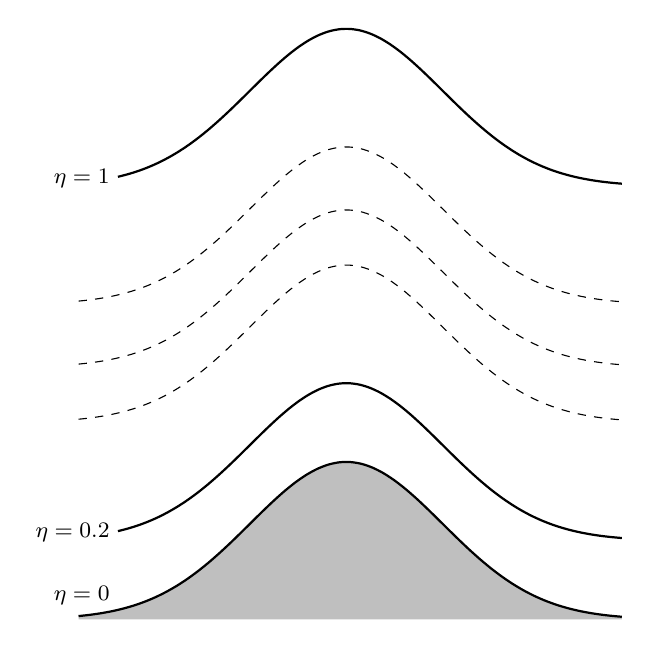
\begin{tikzpicture}[declare function={g(\x)=2*exp(-\x*\x/3);
            xmax=3.5;xmin=-3.4;x0=1.5;ymax=2.75;}]
            \footnotesize
             % \draw[gray!50] ;
             \fill[gray!50] plot[domain=xmin:xmax,samples=15,smooth] (\x,{g(\x)}) -- (xmax,0) -| cycle;  
             \draw [thick]  plot[domain=xmin     :xmax,samples=51,smooth] (\x,{g(\x)}); 
             \draw [thick]  plot[domain=xmin+0.5:xmax,samples=51,smooth] (\x,{1+g(\x)}); 
             \draw [dashed] plot[domain=xmin     :xmax,samples=51,smooth] (\x,{2.5+g(\x)}); 
             \draw [dashed] plot[domain=xmin     :xmax,samples=51,smooth] (\x,{3.2+g(\x)}); 
             \draw [dashed] plot[domain=xmin     :xmax,samples=51,smooth] (\x,{4+g(\x)}); 
             \draw [thick]  plot[domain=xmin+0.5 :xmax,samples=51,smooth] (\x,{5.5+g(\x)}); 
             \draw (xmin+0.5,0.3) node[left] {$\eta=0$} ;
             \draw (xmin+0.5,1.1) node[left] {$\eta=0.2$} ;
             \draw (xmin+0.5,5.6) node[left] {$\eta=1$} ;
        \end{tikzpicture}
    \end{minipage}%
    \begin{minipage}[b]{.5\textwidth} % right
      \centering
        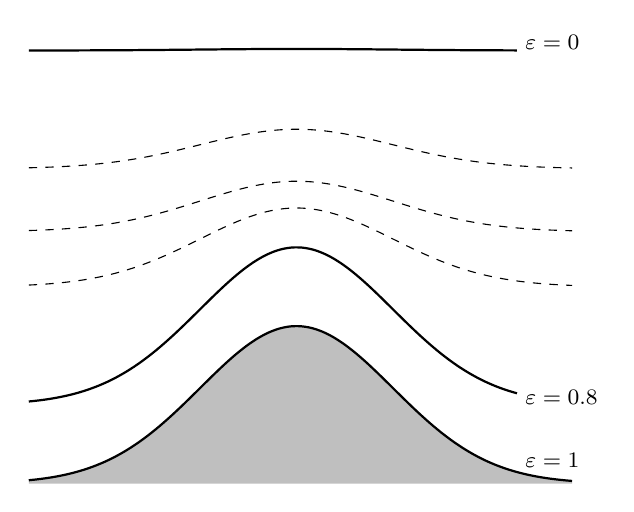
\begin{tikzpicture}[declare function={g(\x)=2*exp(-\x*\x/3);
            xmax=3.5;xmin=-3.4;x0=1.5;ymax=2.75;}]
            \footnotesize
             % \draw[gray!50] ;
             \fill[gray!50] plot[domain=xmin:xmax,samples=15,smooth] (\x,{g(\x)}) -- (xmax,0) -| cycle;  
             \draw[thick]   plot[domain=xmin:xmax    ,samples=51,smooth] (\x,{g(\x)}); 
             \draw[thick]   plot[domain=xmin:xmax-0.7,samples=51,smooth] (\x,{1.0+     g(\x)}); 
             \draw[dashed]  plot[domain=xmin:xmax    ,samples=51,smooth] (\x,{2.5+ 0.5*g(\x)}); 
             \draw[dashed]  plot[domain=xmin:xmax    ,samples=51,smooth] (\x,{3.2+0.32*g(\x)}); 
             \draw[dashed]  plot[domain=xmin:xmax    ,samples=51,smooth] (\x,{4.0+0.25*g(\x)}); 
             \draw[thick]   plot[domain=xmin:xmax-0.7,samples=51,smooth] (\x,{5.5+0.01*g(\x)}); 
             \draw (xmax-0.7,0.3) node[right] {$\varepsilon=1$} ;
             \draw (xmax-0.7,1.1) node[right] {$\varepsilon=0.8$} ;
             \draw (xmax-0.7,5.6) node[right] {$\varepsilon=0$} ;
        \end{tikzpicture}
    \end{minipage}
    \caption{\label{fig:ch9.3} Схематичный пример орографической $\eta$-координаты (слева) и гибридной $\varepsilon$-координаты справа}
    \end{figure}
    
Приведем в качестве примера одну из таких координат, которая записывается в виде
    \begin{equation}
    \label{eq:hybridframe}
        \varepsilon= \sigma_{\varepsilon_s} =
        \underbrace{\left( \frac{p-p_T}{p_s-p_T} \right)}_{\sigma}
        \underbrace{\left( \frac{p_r(z_s) - p_T}{p_r(0) - p_T} \right)}_{\varepsilon_s}
    \end{equation}
Первый множитель здесь -- стандартная $\sigma$-система, $p_s$ -- давление у поверхности, $p_T$ -- давление на верхней границе области, $p_r(z_s)$ -- давление на данной высоте в стандартной атмосфере, $p_r(0)$ -- давление на уровне моря в стандартной атмосфере. 

Нетрудно заметить, что при высоте $z_s\rightarrow0$ $\varepsilon_s\rightarrow1$ и в (\ref{eq:hybridframe}) $\varepsilon\rightarrow\sigma$. При более общей ситуации член 
    \begin{equation*}
         \frac{p_r(z_s) - p_T}{p_r(0) - p_T} 
    \end{equation*}
не очень далек от единицы (настолько, насколько давление у поверхности земли в данный момент времени отличается от стандартного). Оставшийся член 
    \begin{equation*}
         \frac{p-p_T}{p_s-p_T}=\frac{p-p_T}{const} 
    \end{equation*}
квазигоризонтален (настолько, насколько отклоняется от нее данная изобарическая поверхность).

   \begin{warn}
        Добавить про вертикальную координату в WRF ($\eta$ и гибридную!) 
   \end{warn}
